% 
% Lecture Template for ME3023 -  Measurements in Mechanical Systems - Tennessee Technological University
%
% Spring 2020 - Summer 2020
% Tristan Hill, May 07, 2020 - June 12, 2020
% Module 4 - Strain Gauges
% Topic 1 - Measuring Strain
%

\documentclass{beamer}                         % for presentation (has nav buttons at bottom)
%\documentclass[handout]{beamer}  % for handout 
\usepackage{beamerthemesplit}
\usepackage{amsmath}
\usepackage{listings}
\usepackage{multicol}
\usepackage{framed}

\beamertemplateballitem

% custom colors
\definecolor{TTUpurple}{rgb}{0.3098, 0.1607, 0.5176} % TTU Purple (primary)
\definecolor{TTUgold}{rgb}{1.0000, 0.8666, 0.0000} % TTU Gold (primary) 
\definecolor{mygray}{rgb}{.6, .6, .6}
\definecolor{mypurple}{rgb}{0.6,0.1961,0.8}
\definecolor{mybrown}{rgb}{0.5451,0.2706,0.0745}
\definecolor{mygreen}{rgb}{0, .39, 0}
\definecolor{mypink}{rgb}{0.9960, 0, 0.9960}

% color commands
\newcommand{\R}{\color{red}}
\newcommand{\B}{\color{blue}}
\newcommand{\BR}{\color{mybrown}}
\newcommand{\K}{\color{black}}
\newcommand{\G}{\color{mygreen}}
\newcommand{\PR}{\color{mypurple}}
\newcommand{\PN}{\color{mypink}}
\newcommand{\OR}{\color{TTU}}
\newcommand{\GD}{\color{TTUgold}}


\setbeamercolor{palette primary}{bg=TTUpurple,fg=TTUgold}
\setbeamercolor{palette secondary}{bg=black,fg=TTUgold}
\setbeamercolor{palette tertiary}{bg=black,fg=TTUpurple}
\setbeamercolor{palette quaternary}{bg=TTUgold,fg=black}
\setbeamercolor{structure}{fg=TTUpurple} % itemize, enumerate, etc
\setbeamercolor{section in toc}{fg=TTUpurple} % TOC sections

%\usefonttheme{professionalfonts}

\newcommand{\Lagr}{\mathcal{L}} % lagrangian

\newcommand{\hspcu}{\underline{\hspace{20mm}}} % large horizontal space w underline
\newcommand{\vspccc}{\vspace{6mm}\\} % large vertical space
\newcommand{\vspcc}{\vspace{4mm}\\}   % medium vertical space
\newcommand{\vspc}{\vspace{2mm}\\}     % small vertical space

\newcommand{\hspcccc}{\hspace{10mm}} % large horizontal space
\newcommand{\hspccc}{\hspace{6mm}} % large horizontal space
\newcommand{\hspcc}{\hspace{4mm}}   % medium horizontal space
\newcommand{\hspc}{\hspace{2mm}}     % small horizontal space

\newcommand{\eqscl}{0.9}     % small horizontal space

\author{ME3023 - Measurements in Mechanical Systems} 

\newcommand{\MNUM}{4\hspace{2mm}} % Module number
\newcommand{\TNUM}{3\hspace{2mm}} % Topic number 
\newcommand{\moduletitle}{Strain Gauges}
\newcommand{\topictitle}{P3500 Strain Indicator} 

\newcommand{\sectiontitleI}{Units of Microstrain}
\newcommand{\sectiontitleII}{Quarter, Half, and Full Configurations}
\newcommand{\sectiontitleIII}{Wiring the P3500}
\newcommand{\sectiontitleIV}{Operating the P3500}
\newcommand{\sectiontitleV}{Modern Solution}

% custom box
\newsavebox{\mybox}

\title{Module \MNUM - \moduletitle}

\date{Mechanical Engineering\vspc Tennessee Technological University}

\begin{document}

\lstset{language=MATLAB,basicstyle=\ttfamily\small,showstringspaces=false}

\frame{\titlepage \center\begin{framed}\Large \textbf{Topic \TNUM - \topictitle}\end{framed} \vspace{5mm}}

% Section 0: Outline
\frame{

\large \textbf{Topic \TNUM - \topictitle} \vspace{3mm}\\


\begin{multicols}{2}
\begin{itemize}

	\item \sectiontitleI		\vspc % Section I
	\item \sectiontitleII 	\vspc % Section II
	\item \sectiontitleIII 	\vspc %Section III
	\item \sectiontitleIV 	\vspc %Section IV
	\item \sectiontitleV 	\vspc %Section V

\end{itemize}

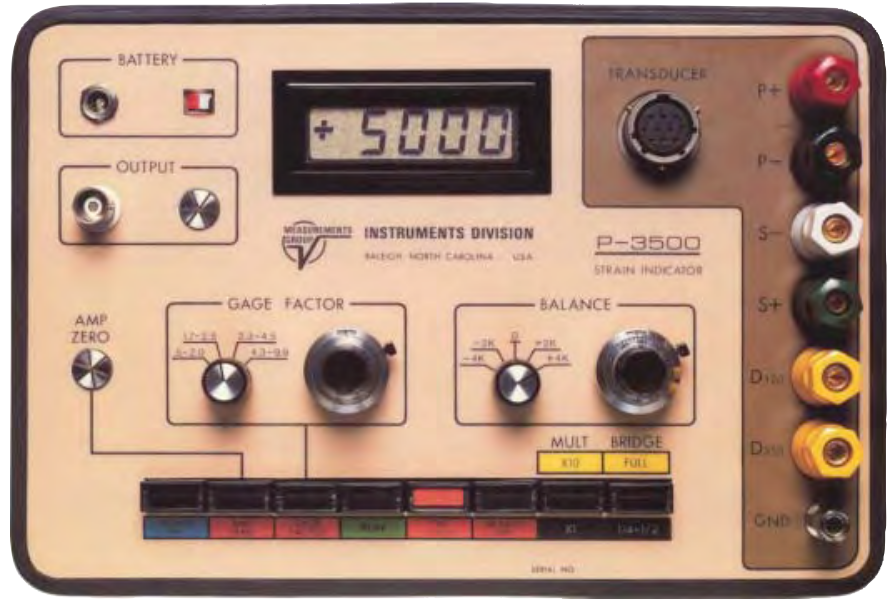
\includegraphics[scale=.18]{p3500_fig1.png}
\end{multicols}

}

% Section I:
\section{\sectiontitleI}

% Section I - Frame I:
\frame{
\frametitle{\sectiontitleI}

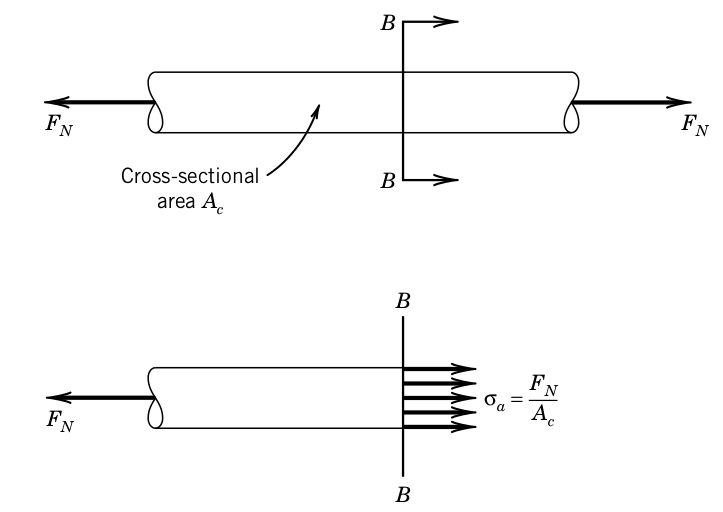
\includegraphics[scale=.25]{strain_fig1.png}

}


% Section II:
\section{\sectiontitleII}

% Section II - Frame I:
\frame{
\frametitle{\sectiontitleII}

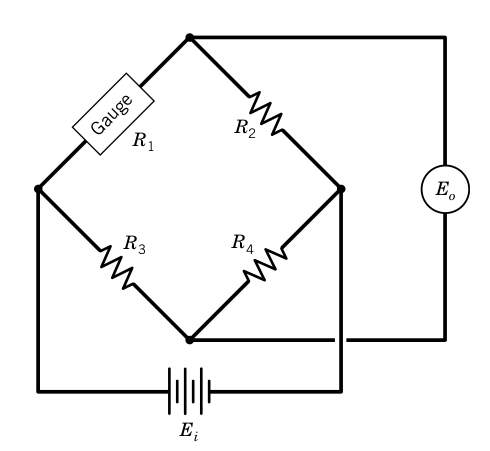
\includegraphics[scale=.2]{gauge_in_bridge_quarter.png} 
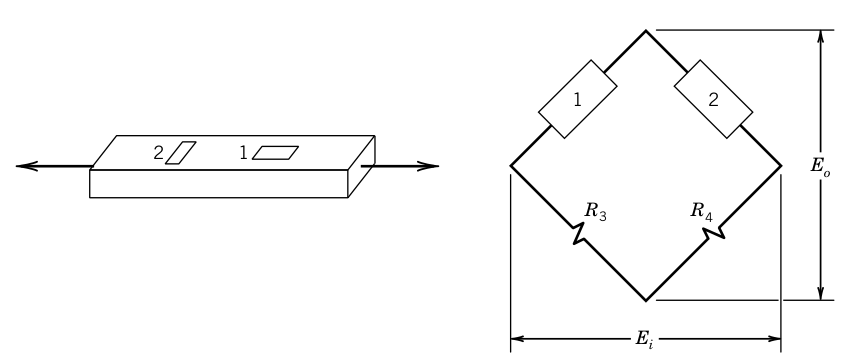
\includegraphics[scale=.2]{gauge_in_bridge_half.png} 
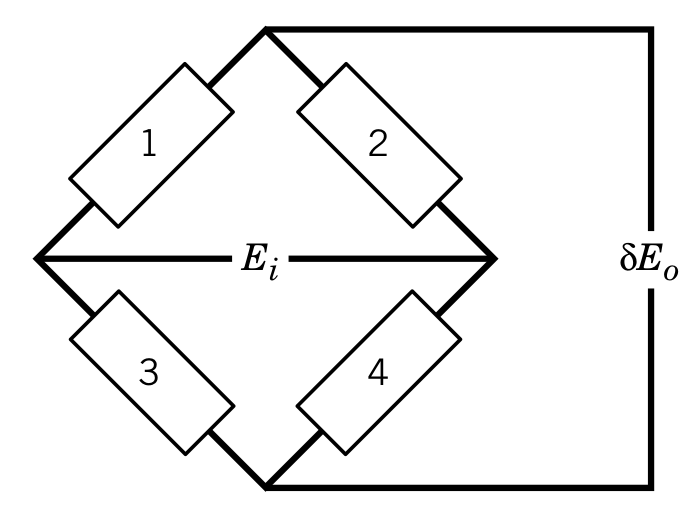
\includegraphics[scale=.16]{gauge_in_bridge_full.png}

}

\frame{
\frametitle{\sectiontitleII}

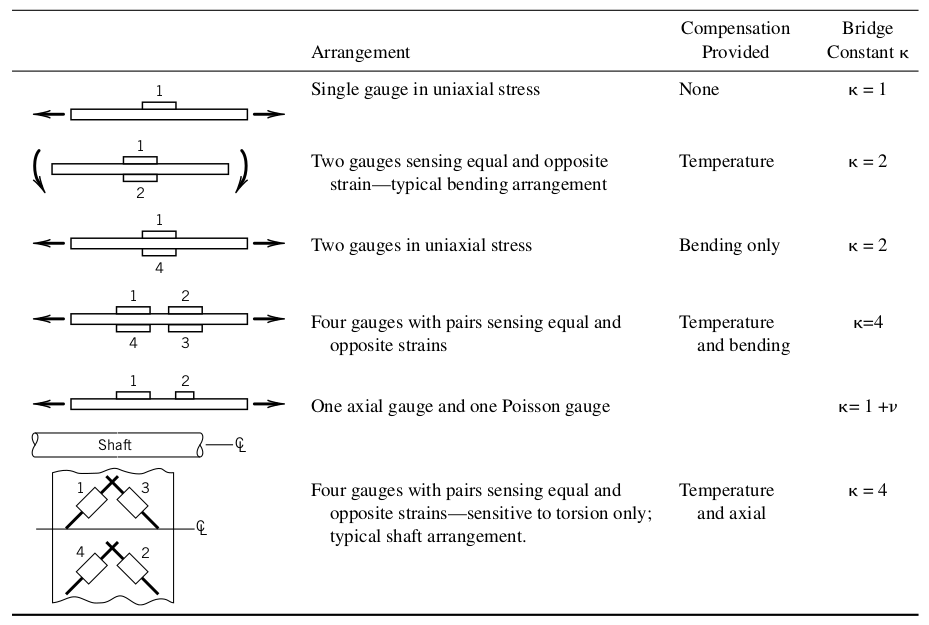
\includegraphics[scale=.3]{gauge_configurations.png}


}

% Section III:
\section{\sectiontitleIII}

% Section I - Frame I:
\frame{
\frametitle{\sectiontitleIII}


\includegraphics[scale=.22]{quarter_half_full.png}


}



% Section IV:
\section{\sectiontitleIV}

% Section I - Frame I:
\frame{
\frametitle{\sectiontitleIV}

\begin{itemize}

\item The instructions are on the unit. 

\item The balancing process is completed after changing any wiring. 

\end{itemize}

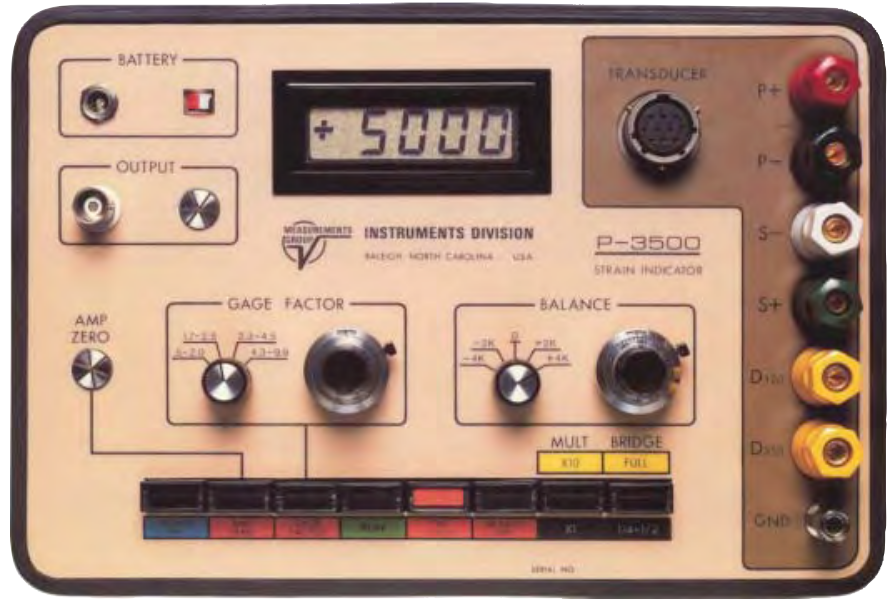
\includegraphics[scale=.228]{p3500_fig1.png}

}

% Section IV:
\section{\sectiontitleV}

% Section I - Frame I:
\frame{
\frametitle{\sectiontitleV}

\begin{itemize}

\item The P3500 is old technology, but still does not mean it is bad.  I have used them myself and they work great. \vspc

\item The manufacturer {\it Vishay Group} has a {\it more} modern solution with DAQ and multiple channels. \vspc

\item There are a variety of low cost options available but be careful.

\begin{itemize}
\item \href{https://learn.sparkfun.com/tutorials/getting-started-with-load-cells/strain-gauge-basics}{Sparkfun - strain gauge basics}
\item \href{https://www.robotshop.com/en/strain-gauge-load-cell-amplifier-shield-2ch.html}{Robot Shop}

\item \href{https://www.elecrow.com/strain-gauge-module-p-735.html}{elecrow}
\end{itemize}

\end{itemize}

}
	
\end{document}





